\chapter{Metodologi}
\label{chap:metodologi}

Pada bagian ini, dijelaskan metode yang digunakan, alat dan bahan penelitian, serta
rancangan implementasi yang digunakan peneliti sebagai kerangka dalam melaksanakan
penelitian yang terstruktur.

\section{Deskripsi Sistem}
\label{sec:deskripsi-sistem}

Penelitian ini menggunakan metode pengembangan sistem yang mengintegrasikan
computer vision, embedded system, dan mekanisme penyerbukan dalam satu kesatuan sistem.
Metode penelitian dirancang untuk menghasilkan prototipe alat penyerbuk kelapa sawit yang
mampu mendeteksi bunga siap serbuk serta memonitor volume pollen secara real-time, dan
selanjutnya diintegrasikan dengan drone sebagai platform pembawa.
Secara umum, alur metode penelitian terdiri dari pengumpulan data, pengembangan
model deteksi berbasis YOLO, perancangan mekanisme penyerbuk, integrasi sensor
monitoring volume pollen, serta evaluasi sistem secara menyeluruh. Tahapan metode disusun
secara berurutan agar setiap komponen sistem dapat diuji dan divalidasi sebelum dilakukan
integrasi penuh.

\begin{figure}[H]
  \centering
  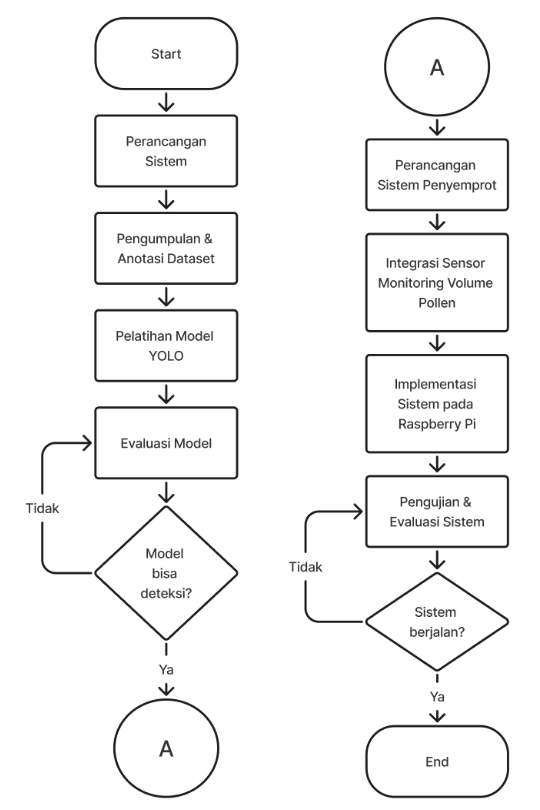
\includegraphics[width=0.3\textwidth]{gambar/flowchart3.png}
  \caption{Diagram Alir Metode Penelitian}
  \label{fig:flowchart3}
\end{figure}

\subsection{Perancangan Sistem}
Tahap awal penelitian adalah perancangan sistem secara keseluruhan, yang bertujuan
untuk menentukan arsitektur sistem dan hubungan antar komponen. Sistem terdiri dari beberapa
komponen utama, yaitu kamera sebagai sensor visual, Raspberry Pi sebagai unit komputasi,
model YOLO sebagai algoritma deteksi objek, blower fan sebagai aktuator penyemprot, sensor
Time of Flight VL53L0X sebagai sensor level pollen, serta integrasi ke drone sebagai platform
pembawa.
Pada tahap ini ditentukan alur kerja sistem, yaitu citra bunga sawit diambil oleh
kamera, kemudian diproses oleh Raspberry Pi menggunakan model YOLO untuk mendeteksi
bunga betina yang siap diserbuki. Ketika objek terdeteksi, sistem akan memeriksa kondisi
volume pollen berdasarkan data sensor. Jika volume pollen mencukupi, mekanisme
penyemprot akan diaktifkan untuk melakukan penyerbukan.

\begin{figure}[H]
  \centering
  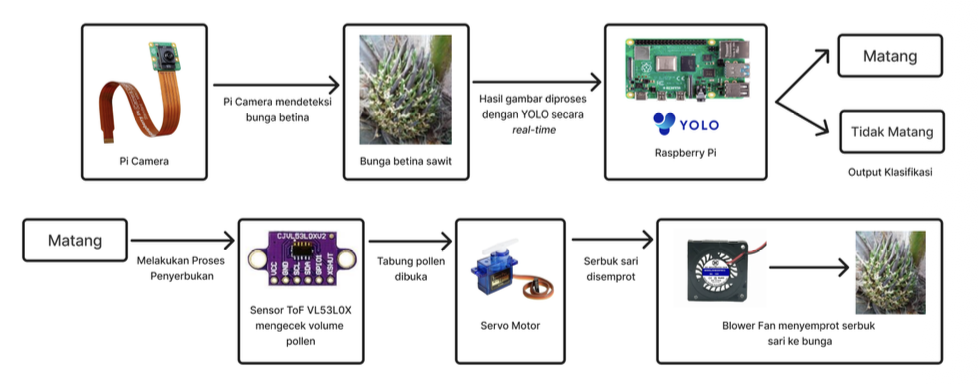
\includegraphics[width=0.6\textwidth]{gambar/alurkerja.png}
  \caption{Alur Kerja Sistem}
  \label{fig:alurkerja}
\end{figure}

\subsection{Pengumpulan dan Anotasi Dataset}
Tahap ini bertujuan untuk memperoleh \emph{dataset} citra bunga kelapa sawit yang digunakan untuk melatih model deteksi. Pengumpulan data dilakukan di kebun kelapa sawit yang berada di Blitar, dengan mengambil citra bunga betina menggunakan kamera HP dan kamera \emph{drone}. Pengambilan data dilakukan berbagai kondisi, seperti perbedaan sudut pandang dan jarak. Selain itu, pengambilan data akan dilakukan pada siang hari agar model bisa memprediksi gambar di saat pengujian nyata. \emph{Dataset} diklasifikasikan menjadi dua kelas inti, yaitu bunga matang dan tidak matang.

Citra yang diperoleh kemudian dianotasi menggunakan perangkat \emph{labeling} seperti Roboflow dengan memberikan \emph{bounding box} pada objek bunga betina. \emph{Dataset} dibagi menjadi data latih, data validasi, dan data uji untuk memastikan proses pelatihan model berjalan optimal dan tidak mengalami \emph{overfitting}.

\subsection{Pelatihan Model YOLO}
Setelah \emph{dataset} siap, tahap berikutnya adalah pelatihan model deteksi menggunakan YOLO. Proses pelatihan dilakukan di Google Colab dengan memanfaatkan GPU untuk mempercepat proses komputasi. \emph{Dataset} yang telah dianotasi digunakan sebagai input pelatihan, sementara parameter pelatihan seperti \emph{learning rate}, \emph{batch size}, dan jumlah \emph{epoch} disesuaikan agar model mencapai performa terbaik.

Perbandingan dilakukan terhadap beberapa varian YOLO berdasarkan parameter ukuran model, waktu inferensi pada Raspberry Pi, serta nilai mAP@0.5 untuk menentukan model yang paling optimal antara akurasi dan kecepatan. Model dengan performa terbaik kemudian diekspor ke format yang kompatibel dengan Raspberry Pi untuk keperluan inferensi \emph{on-device}.

\subsection{Evaluasi Model YOLO}
Pada tahap evaluasi model, dilakukan perbandingan beberapa varian arsitektur YOLO untuk menentukan model yang paling optimal digunakan pada \emph{edge device} (Raspberry Pi 5). Model yang dibandingkan meliputi YOLOv8, YOLOv9, YOLOv10, YOLOv11, dan YOLO26 dengan pertimbangan model tersebut termasuk dalam kategori \emph{lightweight object detector} yang umum digunakan untuk aplikasi \emph{real-time}.

\subsection{Perancangan Sistem Penyemprot}
Mekanisme penyerbuk dirancang menggunakan sistem tabung penyimpanan \emph{pollen} yang dilengkapi aktuator \emph{servo motor} sebagai mekanisme buka-tutup katup (\emph{valve control}). \emph{Servo motor} dikendalikan oleh Raspberry Pi melalui sinyal PWM untuk mengatur durasi pembukaan katup sehingga volume \emph{pollen} yang dikeluarkan dapat dikontrol secara presisi.

Mekanisme ini menggunakan konsep \emph{controlled release}, di mana katup hanya terbuka ketika model YOLO mendeteksi bunga pada fase reseptif dan volume \emph{pollen} terdeteksi mencukupi. Setelah durasi tertentu (misalnya 1--3 detik), katup akan tertutup kembali untuk mencegah pemborosan \emph{pollen}. Setelah itu, \emph{blower fan} akan meniupkan udara agar \emph{pollen} keluar dan menyerbuki bunga betina kelapa sawit.

\subsection{Integrasi Sistem Monitoring Volume Pollen}
Sistem \emph{monitoring} volume \emph{pollen} diintegrasikan menggunakan sensor \emph{Time of Flight} (ToF) VL53L0X yang dipasang pada bagian atas tabung \emph{pollen} untuk mengukur jarak permukaan \emph{pollen} secara non-kontak. Nilai jarak yang diperoleh dikonversi menjadi tinggi dan volume \emph{pollen} berdasarkan dimensi tabung yang telah ditentukan. Data volume ini digunakan sebagai parameter untuk memastikan ketersediaan \emph{pollen} sebelum proses penyerbukan buatan dilakukan.

Hasil \emph{monitoring} volume \emph{pollen} diintegrasikan dengan sistem kendali aktuator, di mana motor \emph{servo} berfungsi sebagai katup pembuka tabung \emph{pollen} dan \emph{blower fan} sebagai media penyemprotan serbuk sari ke bunga betina sawit. Proses penyerbukan hanya dijalankan apabila volume \emph{pollen} memenuhi ambang batas minimum, sehingga integrasi ini menjamin proses penyerbukan berlangsung secara otomatis, terkontrol, dan efisien.

\subsection{Implementasi Sistem pada Raspberry Pi}
Tahap integrasi dilakukan dengan menggabungkan model deteksi berbasis YOLO, sistem \emph{monitoring} volume \emph{pollen}, serta mekanisme aktuator buka-tutup tabung \emph{pollen} ke dalam satu sistem terpadu pada Raspberry Pi 5. Kemudian sistem diintegrasikan pada \emph{drone quadcopter} kelas ringan menggunakan dudukan hasil cetak 3D yang dirancang khusus agar tidak mengganggu pusat massa dan kestabilan penerbangan.

\emph{Drone} yang digunakan memiliki konfigurasi empat baling-baling (\emph{quadcopter}) dengan dimensi bentang diagonal $\pm$180--220 mm dan berat kosong di bawah 500 gram. Selain mempertimbangkan distribusi massa perangkat, pemilihan baterai juga disesuaikan dengan kapasitas \emph{payload drone}. Kapasitas \emph{payload} tambahan diperkirakan berada pada kisaran 150--250 gram agar rasio \emph{thrust-to-weight} tetap stabil untuk manuver jarak dekat di area perkebunan. Sistem penyerbuk yang dikembangkan terdiri dari beberapa komponen utama dengan estimasi berat seperti Raspberry Pi 5 sekitar 46 g, kamera sekitar 10 g, blower fan ±40 g, servo motor ±20 g, sensor VL53L0X ±3 g, serta mekanisme tabung pollen dan dudukan 3D printing sekitar 50–70 g. Dengan demikian total estimasi berat sistem berada pada kisaran 170–190 gram.

\begin{figure}[H]
  \centering
  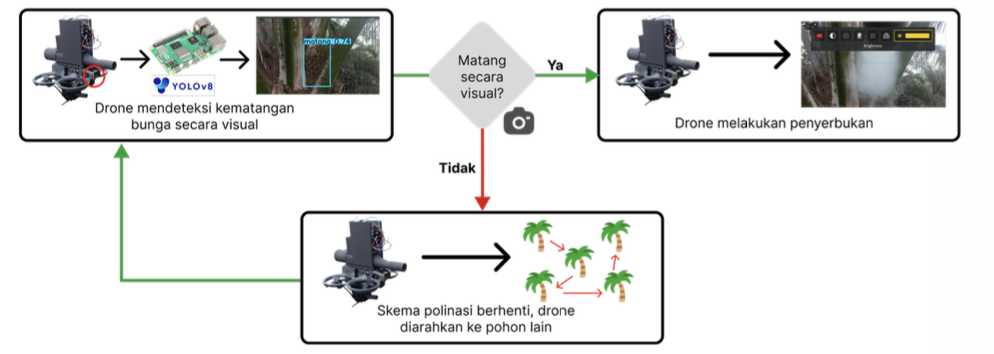
\includegraphics[width=0.6\textwidth]{gambar/carakerjadrone.png}
  \caption{Diagram Cara Kerja Sistem dengan Integrasi Kepada Drone}
  \label{fig:carakerjadrone}
\end{figure}

Untuk menyuplai daya sistem digunakan baterai Li-Po 2S (7.4 V) dengan kapasitas 1000–1500 mAh yang memiliki berat sekitar 80–110 gram. Baterai ini dipilih karena memiliki rasio energi terhadap berat yang tinggi serta ukuran fisik yang masih kompatibel dengan ruang pemasangan pada drone kelas ringan. Penempatan baterai dirancang sedekat mungkin dengan pusat massa drone agar distribusi berat tetap seimbang dan tidak mempengaruhi kestabilan penerbangan. Dengan mempertimbangkan total berat sistem dan baterai yang masih berada dalam batas payload drone, integrasi perangkat diharapkan tetap memungkinkan operasi drone yang stabil selama proses penyerbukan.

\subsection{Pengujian & Evaluasi Sistem}
Evaluasi dilakukan untuk mengukur kinerja sistem secara menyeluruh. Parameter evaluasi meliputi akurasi deteksi bunga sawit oleh model YOLO, respons sensor terhadap perubahan volume pollen, keandalan mekanisme penyemprotan, serta kestabilan sistem saat dipasang pada drone. Pengujian dilakukan dalam dua tahap, yaitu pengujian statis dengan menggunakan alat yang terbatas dan pengujian langsung di kebun sawit. Hasil evaluasi digunakan untuk menilai keberhasilan sistem serta mengidentifikasi potensi pengembangan lanjutan.

\section{Implementasi Alat}
\label{sec:implementasi-alat}

Alat diimplementasikan dengan \lipsum[1]

% Contoh pembuatan potongan kode
% \begin{lstlisting}[
%   language=C++,
%   caption={Program halo dunia.},
%   label={lst:halodunia}
% ]
% #include <iostream>

% int main() {
%     std::cout << "Halo Dunia!";
%     return 0;
% }
% \end{lstlisting}

\lipsum[2-3]

% Contoh input potongan kode dari file
\lstinputlisting[
  language=Python,
  caption={Program perhitungan bilangan prima.},
  label={lst:bilanganprima}
]{program/bilangan-prima.py}

\section{Skenario Eksperimen dan Baseline}
\label{subsec:skenario-eksperimen}

Untuk memvalidasi metrik di atas, sistem usulan dibandingkan dengan \textit{baseline} standar industri sebagaimana dirangkum dalam Tabel \ref{tab:skenario-baseline}.

\begin{table}[!ht]
\centering
\footnotesize
\caption{Rangkuman Skenario Eksperimen dan Baseline}
\label{tab:skenario-baseline}
\begin{tabular}{|p{3cm}|p{4cm}|p{4cm}|}
\hline
\textbf{Parameter Evaluasi} & \textbf{Baseline (Kontrol)} & \textbf{Sistem Usulan} \\
\hline
\textit{Time to First Command} (ms) & \textit{MicroVM Cold Start}: Menjalankan agen dengan MicroVM standar (\textit{fresh boot}). & \textit{MicroVM Snapshot Restore}: Memulihkan MicroVM dari kondisi \textit{pre-initialized}.\\
\hline
\textit{Accuracy} (\%) & \textit{Static/Reactive}: Tidak ada prediksi (0\% proactive). Mengandalkan instalasi saat jalan. & \textit{Context-Aware}: Memprediksi kebutuhan lingkungan sebelum eksekusi. \\
\hline
\textit{Task Done} (s) & \textit{Reactive Provisioning}: Waktu tugas ditambah waktu unduh dan instalasi alat. & \textit{Proactive Provisioning}: Hanya waktu tugas (Waktu instalasi $\approx$ 0). \\
\hline
\textit{Storage} (MB) & \textit{Full MicroVM Snapshot}: Menyalin seluruh memori dan disk setiap sesi. & \textit{Incremental Snapshot}: Hanya menyimpan delta (\textit{Copy-on-Write}). \\
\hline
\end{tabular}
\end{table}

